\chapter{Packet Loss}
\label{chap:PacketLoss}
\head{Some considerations when make remote control computations over a \ac{RF} link.}

\noindent One of the features of the Kalman-filter is that it makes it possible to have a better reaction to a missing packet. This comes from the fact that a missing packet can merely be treated as a packet with very high noise, meaning a Kalman gain of 0. With a Kalman gain of 0, the measurement included in the packet will not be included in the next prediction. This is a key feature of the filter as well as a key feature of the project.

If a \ac{GPS} measurement is lost the ship is effectively sailing blindfolded. If however measurements of other parameters are available, it is possible to very effectively predict where the ship is positioned and which heading it has. With this information it is possible to still control the ship, remotely, until a new fix is received. This makes the system robust in regards to packetloss, as it is estimated that only a limited amount of the packets will be lost. 

If we assume that 10$\%$ of the packets will be lost, regardless of the type, we can estimate the approximate average sampling rate. This can be calculated from equation (\ref{eq:packetloss}). This is quickly observable by the fact that a packetloss of 0 results the actual sampling rate, a packetloss of 50$\%$ results in half the sampling rate, and a packetloss of 100$\%$ results in an 0 sampling rate.
\begin{equation}
\hat{f_s} = f_s(1-p)
\label{eq:packetloss}
\end{equation}

\begin{tabbing}
Where \= $\hat{f_s}$ is the effective average sampling speed\\
\> $f_s$ is the actual sampling speed\\
\> $p$ is the probability for packet loss
\end{tabbing}
From this it can be seen that a system implementing this form of Kalman filtering as a way to deal with packetloss can effectively be estimated as a lossless system with a lower sampling rate.

It can also be seen that there are two ways to generate a better estimate -- reduce the probability of packetloss or increase the sampling rate.
If we assume a fixed samplingrate we can estimate $p$ and, in many cases, decrease it by increasing the signal strength. If an estimate of $p$ is achieved, the actual sampling rate can be calculated by giving a desired effective sampling rate and calculating the necessary requirement.

 As seen in \todo{ref chapter with considerations about worse estimates during turning} the estimates become worse when the ship is turning. This can be mediated by turning up the signal strength to reduce the probability of packet loss, and therefore increasing the effective average sampling rate. 

The packetloss can be handled by having a matrix with the index on the diagonal corresponding to a given type of sample being either 1 or 0, depending on whether a sample is available. Multiplying this with the Kalman gain matrix, B, will set the corresponding column to 0, which is what is desired.

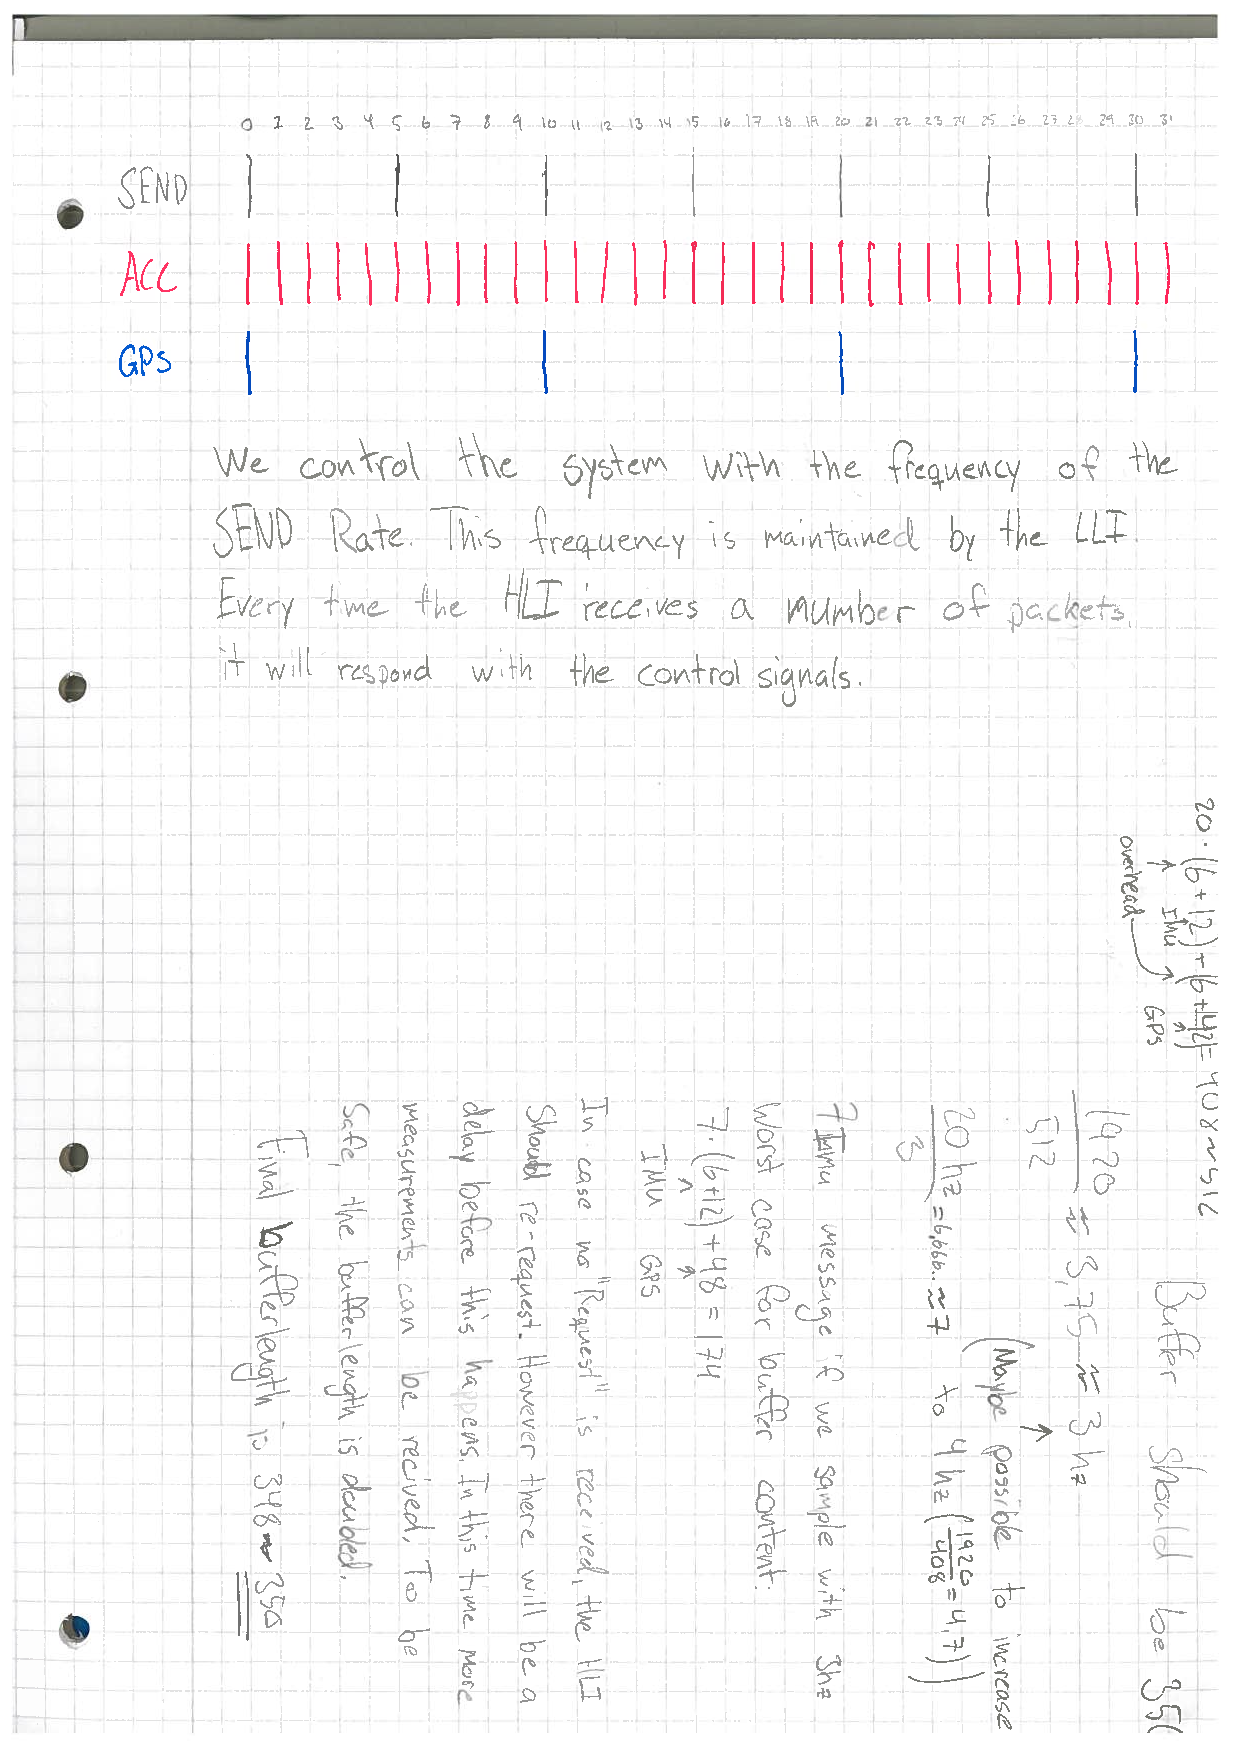
\includegraphics[width = \textwidth]{simplex}
